\section{Introduction}
In this section, we will discuss about the goal of the project, the different component used, the assumptions and model taken.

\subsection{Goal of this project}
The aim of this project was to design and implement an embedded system. To do so, we decided to create an Arduino controller for a traffic light crossroad. In this system, many hypothesis regarding the crossroad properties will be taken and will be explain more deeply in the next sections.
We also decided to join the Embedded Software project and the Formal verification of computer systems project. We will, in this report, clearly state the differences about the two projects to point out what we did differently for those two project.

\subsection{Crossroad assumptions}
\begin{figure}[!ht] \label{fig:crossroad}
  \centering
    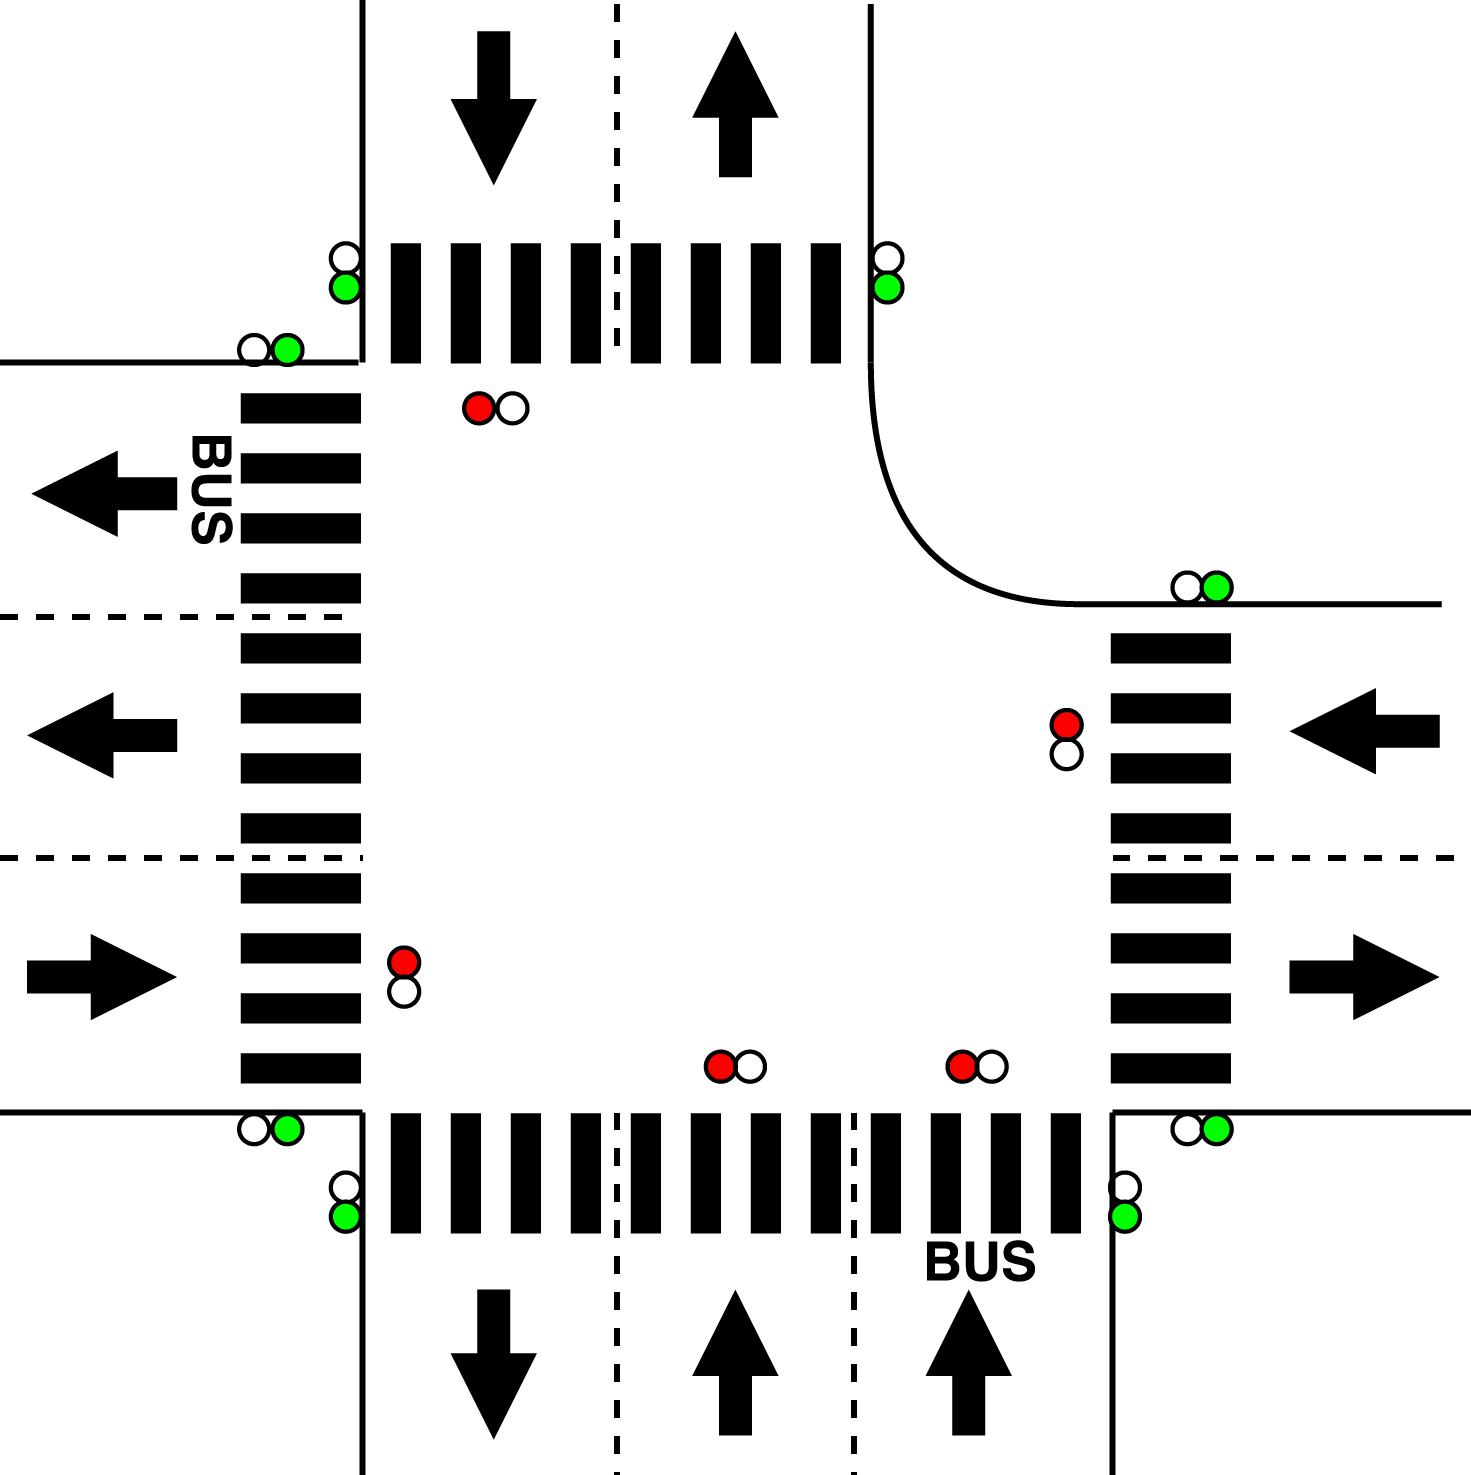
\includegraphics[width=0.7\textwidth]{picture/crossroad.png}
    \caption{The crossroad model}
\end{figure}

Before defining the different actors and components in our system, some important assumptions about our model have to be taken:
\begin{itemize}
    \item The different vehicles will respect the Highway Code. This for example means that if a car is turning right and there are pedestrians crossing, the car will stop to let them pass and will turn after.
    \item At any time, a pedestrian can push a button to cross the street. If there are many pedestrians pushing the button, the first push will only be considered. This means, in our assumptions that more pedestrians are only joining the first one.
    \item The pedestrians will cross the street within the given time. This also means that they follow the laws and rules.
    \item As for the pedestrians, the vehicles will also cross the street within a given time.
\end{itemize}

\subsection{Actors}
In this section, the different actors interacting with the system will be looked at. There will be pedestrians, buses and traffic lights.

\subsubsection{Pedestrians}
As shown on Figure \ref{fig:crossroad}, there are four different crosswalks in our model.  To make a call for the pedestrians to cross, a push button has been implemented on the controller. This means that when one pedestrian has pushed one of the button of the crossroad, the call has been made for all the pedestrians from all the sides of it. When the call is accepted by the system, the pedestrians can walk freely in the crossroad because all the lights for the cars and the buses will be red. This also means that if no pedestrians are pushing the button, meaning that no pedestrians are present, their traffic lights will always be red so the cars will always be able to drive through the crossroad.
To summarize, when the pedestrians can cross, no other vehicles can drive and have thus to wait for the red light to be green. 

\subsubsection{Buses}
The buses in our model can only go from the South path of the crossroad to the West part of it. Those buses will be created thanks to an outside event, like a push button. When a bus is coming, it will have absolute priority on every other actors. This means that when a bus has arrived in the crossroad, because it as to go through all the other lanes, the traffic lights for everyone have to be red.

\subsubsection{Traffic Lights}
In our embedded systems, traffic lights can be green, orange or red as in the real life. We consider that when a traffic light is green, cars are going through the crossroad and respect the Highway Code. Cars are thus, in our model, not really an actor since they are not created, we just assume them to pass through the crossroad when their traffic lights are green. 
There are some assumptions we made about the traffic lights that are important, because we wanted fairness in our system. For example, even if the pedestrians can always push the button to have the ability to walk through the crosswalk, they have to wait that at least all other traffic lights for the cars have been green once. This means that, if no buses come and pedestrians are always pushing the button, the crosswalk with allow the cars of each side to ride once before the pedestrians can cross again. Thanks to that, each elements in the model can have the green light $\frac{1}{3}$ of the time.
Another assumption is that when the South light is green, the North light is also green. On the contrary, when the East light is green, the West light is green. This means that South-North and East-West will be synchronized lights.

\subsubsection{Connection with Formal Verification}
We decided to combine those two projects together because they follow the same basic idea and because they are also complementary. When we look at the embedded project, we had to modelize an environment, and generate a controller based on that model to avoid unwanted situations through winning strategies, computed with timed games. For the formal verification course, a more formal approach was taken. We also had to modelize the system using UPPAAL, but also to verify that the model was compliant to some specific properties. 

\subsection{Why using verification on a small embedded system}
It is not always the best idea to write the code for the controller, to test it using unit test and the to set it up on an embedded system. Indeed, one could imagine what could happen if the code of the controller is wrong in a crossroad, meaning that all the traffic lights could be green at the same time leading to possible car accident. This is why we first want to model the system as a smaller system to verify if the propreties are respected. Thanks to this, the risk of having an accident can be reduced since we test if no unwanted states can be reached. This is why formal verification of small embedded systems can be really useful.
